\documentclass{homework}
\class{Stage 2 Mathematical Methods}
\author{SACE ID: 799157J}
\title{\Large{Ratios of Areas of a Quartic Function}}
\date{\today}
\usepackage{tabularx}
\usepackage{paracol}
\usepackage{fancyhdr}
\pagestyle{fancy}
\cfoot{\thepage}
\usepackage{tikz}
\usepackage{array,polynom}
\usepackage{floatrow}
% Table float box with bottom caption, box width adjusted to content
\newfloatcommand{capbtabbox}{table}[][\FBwidth]
\usepackage{blindtext}
\usepackage{polynom}
\makeatletter
\def\pld@CF@loop#1+{%
    \ifx\relax#1\else
        \begingroup
          \pld@AccuSetX11%
          \def\pld@frac{{}{}}\let\pld@symbols\@empty\let\pld@vars\@empty
          \pld@false
          #1%
          \let\pld@temp\@empty
          \pld@AccuIfOne{}{\pld@AccuGet\pld@temp
                            \edef\pld@temp{\noexpand\pld@R\pld@temp}}%
           \pld@if \pld@Extend\pld@temp{\expandafter\pld@F\pld@frac}\fi
           \expandafter\pld@CF@loop@\pld@symbols\relax\@empty
           \expandafter\pld@CF@loop@\pld@vars\relax\@empty
           \ifx\@empty\pld@temp
               \def\pld@temp{\pld@R11}%
           \fi
          \global\let\@gtempa\pld@temp
        \endgroup
        \ifx\@empty\@gtempa\else
            \pld@ExtendPoly\pld@tempoly\@gtempa
        \fi
        \expandafter\pld@CF@loop
    \fi}
\def\pld@CMAddToTempoly{%
    \pld@AccuGet\pld@temp\edef\pld@temp{\noexpand\pld@R\pld@temp}%
    \pld@CondenseMonomials\pld@false\pld@symbols
    \ifx\pld@symbols\@empty \else
        \pld@ExtendPoly\pld@temp\pld@symbols
    \fi
    \ifx\pld@temp\@empty \else
        \pld@if
            \expandafter\pld@IfSum\expandafter{\pld@temp}%
                {\expandafter\def\expandafter\pld@temp\expandafter
                    {\expandafter\pld@F\expandafter{\pld@temp}{}}}%
                {}%
        \fi
        \pld@ExtendPoly\pld@tempoly\pld@temp
        \pld@Extend\pld@tempoly{\pld@monom}%
    \fi}
\makeatother
\pagenumbering{arabic}
\begin{document} \maketitle
   \textbf{\large{Introduction}} \vspace{1em}\\ 
A quartic is a fourth degree polynomial with general form $f(x)=ax^4+bx^3+cx^2+dx+e,\,a\neq 0$. Quartics have applications in fields involving computational geometry, including computer graphics, computer-aided design (Shifrin 2013) and optics (O’Connor 1999).  \vspace{0.8em}\\
\begin{paracol}{2}
 When a quartic has 2 inflection points (change in concavity and $f''(x)=0$) and positive leading coefficient, it graphically resembles a W shape (Figure 1). \vspace{0.8em}\\
 A line is drawn through inflection points Q and R, known as $g(x)$. $g(x)$ meets the quartic at 2 other points P and S. The equation of the tangent at Q meets the quartic again at point M. \vspace{0.8em}\\
Knowledge of these features allow areas A, B, C, D to be found. The aim of this investigation is to examine the ratio between $A, B, C, D$ for all W shaped quartics, and generalise the ratio through a proof if possible.
\switchcolumn
\begin{figure}[htp]
    \centering
    \includegraphics[width=9cm]{w shaped quartic.png}
    \caption{A W-shaped quartic with all relevant points labelled}
    \label{fig:quartic}
\end{figure}
\end{paracol}
Initially, the area ratios and key features were found for symmetrical W shaped quartics belonging to the family $f(x)=x^4-2ax^3+a^3x,\,a\neq0$. \vspace{0.8em}\\
Test cases for positive integer, positive irrational, and negative rational were used to aid the formation of conjectures regarding key features of $f(x)$ and hence $A:B:C:D$. \vspace{0.8em}\\
Such conjectures were proven or disproven using algebra and calculus. 
Subsequently, other quartics not of the family were investigated to determine if this area ratio holds for all W shaped quartics. An attempt was then made to generalise the conjecture for all W shaped quartics through a proof.\\
\vspace{1.6em}
\begin{center}
\textbf{\large{Investigating the relationship between A, B, C, D for $f(x)= x^4-4x^3+8x+5$}}
\end{center} 
\columnratio{0.5}
\vspace{1.3em}
Before the general form of a symmetrical W shaped quartic is investigated, 
some example functions will be examined. \vspace{0.8em} \\
The first example, $ f(x)= x^4-4x^3+8x+5 $ is a W shaped quartic with integer coefficients. It belongs to the family $x^4-2ax^3+ax^3$, as $a=2$ and the constant term merely translates the quartic up by 5 units. \vspace{0.8em} \\
A range of algebraic concepts, including polynomial long division, the factor theorem, the quadratic formula and binomial expansion, will be used to find the key features of $f(x)$ and the areas A, B, C, D. To find the inflection points Q and R, differential calculus is used. 
\newpage
\begin{flushleft}
\begin{paracol}{2}
    Using the power rule $\frac{d}{dx}(x^{n})=nx^{n-1}$ \vspace{0.4em} \\
    $ f(x)= x^4-4x^3+8x+5 $\vspace{0.4em} \linebreak 
    $\Rightarrow f'(x)=4x^3-12x^2+8 $\vspace{0.4em} \linebreak 
    $\Rightarrow f''(x)=12x^2-24x $ \vspace{1.4em} 
    \linebreak 
    The x-coordinates of Q and R occur when $f''(x)=0 \vspace{0.4em} \linebreak
    \Rightarrow 12x^{2}-24x=0 \vspace{0.4em} \linebreak
    \Rightarrow 12x(x-2)=0 \hspace{1.4em}
    \Rightarrow x=0,2  \vspace{0.4em} \linebreak
    \therefore Q(0, f(0)) $ \text{and} $ R(2, f(2)) $  \vspace{1.4em} \\
    \text{Finding the y-coordinates of Q and R:} \vspace{0.4em} \linebreak
    $ f(0)= 0^4-4(0)^3+8(0)+5=5$ \vspace{0.4em}  \linebreak
     $f(1)= 2^4-4(2)^3+8(2)+5=5$ \vspace{0.4em}  \linebreak 
      $ \therefore Q(0, 5) $ and $R(2, 5)$ \vspace{1.4em} \\
      Although $f''(0)=0$ and $f''(2)=0,$ Q and R are only inflection points if there is a change in concavity. By creating a sign diagram $f''(x)$, a sign change at $x=0,2$ will show a concavity change for $f(x)$ at Q and R. \vspace{1.4em} \\
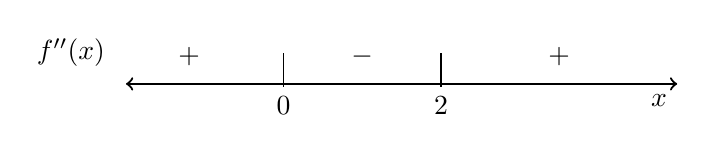
\begin{tikzpicture} 
\draw[thick](-2.7,0.7)node[anchor=north]{$f''(x)$};
\draw[thick,<->] (-2,0) -- (5,0) node[anchor=north east] {$x$};
\foreach \x in {0,2}
   \draw (\x cm,1.1em) -- (\x cm,-1pt) node[anchor=north] {$\x$};
\draw[thick] (-1.2,0.6)node[anchor=north]{$+$};
\draw[thick] (1,0.6)node[anchor=north]{$-$};
\draw[thick] (3.5,0.6)node[anchor=north]{$+$};
\end{tikzpicture} \\
\vspace{1.4em}
   As Q and R have the same y-coordinate of 5, the horizontal line $g(x)=5$ meets both points of inflection (Figure 2). \vspace{0.7em}
   \switchcolumn
\begin{figure}[htp]
    \centering
    \includegraphics[width=7cm]{g2.png}
    \caption{Graphs of $y=f(x)$, $y=g(x)$, and $f(x)$ inflection points Q and R}
    \label{fig:g2}
\end{figure}
\switchcolumn
  \vspace{0.8em}From Figure 2, $y=g(x) $ intersects $y=f(x)$ at two additional points. Let these points be P and S.
    \linebreak \linebreak
    The x-coordinates of P and S are found by equating $f(x)$ and $g(x)$. \vspace{0.5em}\\ 
    $\Rightarrow x^4-4x^3+8x+5=5 $ \vspace{0.5em}\\
    $\Rightarrow x^4-4x^3+8x=0$\vspace{0.5em} \\
    However, $x=0$ and $x=2$ are known roots of this polynomial, as these are the x-coordinates of Q and R.  \vspace{0.9em}\\
    By the Factor Theorem (Sehgal 2009, p. 119): \vspace{0.5em}\\
    $P(a)=0 \Leftrightarrow (x-a)$ is a factor \vspace{0.5em}\\
    $ \therefore x(x-2)$ is a factor of this polynomial. 
     \switchcolumn
     The x-coordinates of P and S are the remaining roots of $x^4-4x^3+8x$. Since $x^2-2x$ is a known factor, $x^4-4x^3+8x$ is further factorised with polynomial division. \vspace{0.8em}\\
    \begin{center}
    \small{\polylongdiv{x^4-4x^3+8x}{x(x-2)}}
    \linebreak
    \end{center}
    $\therefore \frac{x^4-4x^3+8x}{x(x-2)}=x^2-2x-4 $ \vspace{1em}\linebreak 
    The roots of the quadratic $x^2-2x-4$, can be found from the quadratic formula $\frac{-\beta\pm \sqrt{\beta^2-4\alpha\gamma}}{2\alpha}$. \vspace{0.8em} \\
    $\Rightarrow x=\frac{2\pm \sqrt{2^2-4(-4)}}{2} 
    \Rightarrow x=\frac{2\pm \sqrt{20}}{2}
    \Rightarrow x=\frac{2\pm 2\sqrt{5}}{2} \vspace{0.7em}\linebreak 
    \therefore x=1+\sqrt{5}, 1-\sqrt{5} \space $
     \linebreak \linebreak
    $\because$ P and S pass through $g(x)=5,$ \\
    $\therefore P(1-\sqrt{5}, 5)  \hspace{1em}S(1+\sqrt{5}, 5)$ \linebreak\linebreak
    Let the function $h(x)$ be the tangent to $f(x)$ at point Q. \linebreak 
    $\Rightarrow h(x)=f'(0)(x-0)+f(0)$ \vspace{0.5em}\\ 
    \small{$\because f'(0)=4(0)^3-12(0)^2+8=8$} \vspace{0.5em}\\  
    \small{$\because f(0)=0^4-4(0)^3+8(0)+5=5$} \vspace{0.5em}\\ 
    \normalsize{$\therefore h(x)=8x+5$} \\ 
    \end{paracol} \newpage
    \begin{paracol}{2}
    \vspace{0.7em} From Figure 1, it is likely that $h(x)$ will intersect $f(x)$ again. 
    This point of intersection is known as M. \vspace{1em}\\
    The x-coordinate of M is found by equating $h(x)$ with $f(x)$. \vspace{0.7em}\\
    $\Rightarrow x^4-4x^3+8x+5=8x+5 $ \vspace{0.7em}\\ 
    $ \Rightarrow x^4-4x^3=0 $ \hspace{2em} 
    $ \Rightarrow x^3(x-4)=0  $ \vspace{0.7em}\\
    $ \therefore x=0, 4  $ \vspace{0.8em} \\
    As $x=0$ is the x-coordinate of Q (Figure 3), $x=4$ is the coordinate of point M. \vspace{0.8em} \\
    $\Rightarrow M(4, h(4)) $\vspace{0.7em}\\
    $h(4)=8(4)+5=32+5=37 \vspace{0.8em}$ \vspace{0.7em}\\
    $\therefore M(4, 37) $ \vspace{1.7em}\\
    \switchcolumn
        \begin{figure}[htp]
        \centering
        \includegraphics[width=8.5cm]{g3.png}
        \caption{Graphs of $y=f(x), y=g(x)$, $y=h(x)$ and points P, Q, R, S and M.}
        \label{fig:g3}
    \end{figure}
  \end{paracol}
\end{flushleft}
\begin{center}
\begin{paracol}{2}
    In Figure 3, the graph of $f(x)$ is shown along with the key features found above.  
    These findings are summarised in the adjacent table and will be used to find areas A, B, C, D as shown in Figure 1. \linebreak \linebreak
    When finding the area between two functions $Y_U$ and $Y_L$, the area is given by $\int_a^{b}[Y_U-Y_L]\, dx$
\switchcolumn
\begingroup
\renewcommand{\arraystretch}{1.3}
    \begin{tabular}{ |c|c| } 
        \hline
        Functions & Points \\
        \hline
        $ f(x)=x^4-4x^3+8x+5 $ & $P(1-\sqrt{5}, 5)$ \\ 
        \hline
        $ g(x)=5 $ & $Q(0, 5)$ \\ 
        \hline
        $ h(x)=8x+5 $ & $ R(2, 5) $ \\ 
        \hline
        {} & $ S(1+\sqrt{5}, 5) $ \\ 
        \hline
        {} & $ M(4, 37) $ \\ 
        \hline
    \end{tabular}
    \endgroup
    \end{paracol}
\end{center} \vspace{1.4em}
\begin{flushleft}
  To find Area A, a definite integral with lower bound 0 and upper bound 2 is used. 
   From Figure 3, $f(x) \text{ is } Y_U$ and $g(x) \text{ is } Y_L$. \linebreak \linebreak
   Area A $=\int_0^{2} x^4-4x^3+8x+5-(5) \, dx$ \vspace{0.4em} \\
   $=\int_0^{2} x^4-4x^3+8x \, dx $ \vspace{0.4em} 
\end{flushleft}
\begin{center}
     Using the Fundamental Theorem of Calculus, $\int_b^a f(x) \, dx = F(a)-F(b)$ \\
\end{center}
\begin{flushleft}
    $ \Rightarrow [\frac{1}{5}x^5-x^4+4x^2]_0^2 $ \vspace{0.4em} \linebreak
    $ \Rightarrow \frac{1}{5}(2)^{5}-(2)^{4}+4(2)^{2}-(\frac{1}{5}(0)^{5}-(0)^{4}+4(0)^{2}) = \frac{32}{5}-16+16=\frac{32}{5} $ \vspace{0.4em} \\ 
    $ \therefore A=\frac{32}{5} \, units^2 $ \vspace{1.4em} \\
\end{flushleft}
\begin{center}
    To find Area B, a definite integral with lower bound 2 and upper bound $1+\sqrt{5}$ will be used. \\
    $g(x)$ is $Y_U$ and $f(x)$ is $Y_L$.
\end{center}
\begin{flushleft}
    Area B = $\int_2^{1+\sqrt{5}} 5-(x^4-4x^3+8x+5) \, dx \linebreak
    = \int_2^{1+\sqrt{5}} -x^4+4x^3-8x \, dx \vspace{0.3em}$ \linebreak
    $\Rightarrow [\frac{-1}{5}x^5+x^4-4x^2]_2^{1+\sqrt{5}}\vspace{0.3em}$ \\
    $\Rightarrow  \frac{-1}{5} (1+\sqrt{5})^5+(1+\sqrt{5})^4-4(1+\sqrt{5})^2 - [\frac{-1}{5} (2)^5+(2)^4-4(2)^2] $ \\
    \newpage
    The Binomial Theorem (Haese 2017) was used to evaluate $(1+\sqrt{5})^5$ and $(1+\sqrt{5})^4$. \vspace{0.4em}\\
    $(1+\sqrt{5})^5=176+80\sqrt{5}$ \hspace{4em} $(1+\sqrt{5})^4=56+24\sqrt{5}$. \hspace{4em} (Appendix A)
    \vspace{0.8em}\\
    $\Rightarrow 
    \frac{-1}{5}(176+80\sqrt{5})+(56+24\sqrt{5})-4(1+2\sqrt{5}+5)+\frac{1}{5}(32)-16+16=\frac{-176-80\sqrt{5}+280+120\sqrt{5}-20-40\sqrt{5}-100}{5}+\frac{32}{5}$ \vspace{0.5em} \\
    $ \Rightarrow  \frac{-16+\sqrt{5}(-80+120-40)}{5} + \frac{32}{5} = \frac{-16+32}{5}=\frac{16}{5} \vspace{1.2em} \hspace{4em}
    \therefore B=\frac{16}{5} \, units^2$ \\
\end{flushleft} 
\begin{center}
    From Figure 3, Area C appears to be equivalent to Area B. This is verified by using a definite integral with lower bound $1-\sqrt{5}$ and upper bound $0$ to find Area C. $g(x)$ is $Y_U$ and $f(x)$ is $Y_L$. \vspace{0.9em}\\
\end{center}
\begin{flushleft}
Area C = $ \int_{1-\sqrt{5}}^0 \, 5-(x^4-4x^3+8x+5) \, dx 
    =\int_{1-\sqrt{5}}^0 \,-x^4+4x^3-8x \, dx =0-[-\frac{1}{5}x^5+x^4-4x^2]_{1-\sqrt{5}}^{0}$
    \vspace{0.5em}\\
    $ = - [\frac{-1}{5} (1-\sqrt{5})^5+(1-\sqrt{5})^4-4(1-\sqrt{5})^2] \vspace{0.5em}$ \vspace{0.4em}\\
    Now, $(1-\sqrt{5})^5$ and $(1-\sqrt{5})^4$ must be expanded. \vspace{0.4em}\\
    $(1-\sqrt{5})^5=176-80\sqrt{5}$ \hspace{4em} $(1-\sqrt{5})^4=56-24\sqrt{5}$. \hspace{4em} (Appendix A)
    \vspace{0.8em}\\
    C = $\frac{1}{5}(176-80\sqrt{5})-(56-24\sqrt{5})+4(1-2\sqrt{5}+5)$
    $=\frac{176-80\sqrt{5}-280+120\sqrt{5}+20-40\sqrt{5}+100}{5}$ \vspace{0.5em} \\
    $C=\frac{176-280+20+100+\sqrt{5}(-80+120-40)}{5}=\frac{16}{5} \hspace{3.4em} \therefore C= \frac{16}{5} \, units^2$ \vspace{1em} \\
\end{flushleft} 
\begin{center}
     Area D is the area between $h(x)$ and $f(x)$ from $x=0$ to $x=4$, where $h(x)$ is $Y_U$ and $g(x)$ is $Y_L$. \\
\end{center}
\begin{flushleft}
\vspace{0.3em}
   Area D $=\int_0^4 \, 8x+5-(x^4-4x^3+8x+5) \, dx $\\
   $\Rightarrow \int_0^4 \, -x^4+4x^3 \, dx  = [\frac{-1}{5}\times x^5-x^4]_0^4 \vspace{0.3em}$ 
   \\
   $\Rightarrow 
   \frac{-1}{5}\times 4^5+4^4 +\frac{1}{5}(0)+0^4=\frac{256}{5}$ \vspace{0.3em}\\
   $\therefore D=\frac{256}{5} \, units^2$ \\
\end{flushleft} 
\begin{center}
    $ \therefore A:B:C:D=\frac{32}{5}:\frac{16}{5}:\frac{16}{5}:\frac{256}{5}=2:1:1:16 $ \vspace{1.3em}\\ 
    \textbf{\large{Investigating areas A, B, C, D for $f(x)= x^4-2ax^3+a^3x$, $a\neq0$}}
\end{center} 
\begin{flushleft}
\vspace{0.7em}
    The quartic previously explored, $f(x)=x^4-4x^3+8x+5$ is a vertical translation of $x^4-2ax^3+a^3x$ $(a=2)$. Two other quartics, $f(x)=x^4-2\pi x^3+\pi^3x$ and $f(x)=x^4+x^3-\frac{1}{8}x$ also belong to this family of quartics, with $a =\pi$ and $\frac{-1}{2}$. \vspace{0.8em}
    \\
    These functions and their relevant features have been graphed on two separate axis (Figure 4)(Figure 5).
\begin{paracol}{2}
\vspace{1.4em}
\renewcommand{\arraystretch}{1.6}
  \begin{tabular}{|c|c|} \hline
  Functions for $a=\pi$ & Points for $a=\pi$ \\ \hline
  $f(x)=x^4-2\pi x^3+\pi^3x$ & $P((\frac{1-\sqrt{5}}{2})\pi, 0)$ \\ \hline
  $g(x)=0$ & $Q(0,0)$ \\ \hline
  $h(x)=\pi^3x$ & $R(\pi, 0)$ \\ \hline
   & $S((\frac{1+\sqrt{5}}{2})\pi,0)$ \\ \hline
   & $M(2\pi,2\pi^4)$ \\ \hline
  \end{tabular}
\switchcolumn
\begin{figure}[htp]
\centering
    \includegraphics[width=8cm]{g4.png}
    \centering
    \caption{Graph of $f(x)=x^4-2\pi x^3+\pi^3x$, $g(x)=0$, $h(x)=\pi^3x$, and points P, Q, R, S, M.}
\end{figure}
\begin{figure}
\includegraphics[width=8.7cm]{g5.png}
\caption{Graph of $f(x)=x^4+x^3-\frac{1}{8}x$, $g(x)=0$, $h(x)=\frac{1}{8}x+\frac{1}{16}$, and points P, Q, R, S, M.}
\end{figure}
\switchcolumn \newpage
\setlength{\tabcolsep}{1.6em}
\renewcommand{\arraystretch}{1.6}
  \begin{tabular}{|c|c|} \hline
  Functions for $a=\frac{-1}{2}$    &   Points for $a=\frac{-1}{2}$\\ \hline
  $f(x)=x^4+x^3-\frac{1}{8}x$ & $P(\frac{1}{4}(-1-\sqrt{5}), 0)$ \\ \hline
  $g(x)=0$ & $Q(\frac{-1}{2},0)$ \\ \hline
  $h(x)=\frac{1}{8}x+\frac{1}{16}$ & $R(0, 0)$ \\ \hline
   & $S(\frac{1}{4}(-1+\sqrt{5}),0)$ \\ \hline
   & $M(\frac{1}{2},\frac{1}{8})$ \\ \hline
  \end{tabular} 
\end{paracol}
    \vspace{1.4em} The areas of A, B, C, D are summarised in the following table. Refer to Appendix A and B for full working.
    \end{flushleft}
\begin{center}
\begingroup
\setlength{\tabcolsep}{3.6em}
\renewcommand{\arraystretch}{1.6}
    \begin{tabular}{ |c|c|c| } 
        \hline
        {} & $f(x)=x^4-2\pi x^3+\pi^3x$ & $f(x)=x^4+x^3-\frac{1}{8}x$ \\
        \hline
        Value of $a$ & $a=\pi$ & {$a=\frac{-1}{2}$} \\
        \hline
        A ($units^2$) & $\frac{\pi^5}{5}$ & {$\frac{1}{160}$} \\
        \hline
        B ($units^2$) & $\frac{\pi^5}{10}$ & {$\frac{1}{320}$} \\
        \hline
        C ($units^2$) & $\frac{\pi^5}{10}$ & {$\frac{1}{320}$} \\
        \hline
        D ($units^2$) & $\frac{8\pi^5}{5}$ & {$\frac{1}{20}$} \\
        \hline 
        $A:B:C:D$ & $2:1:1:16$ & $2:1:1:16$ \\
        \hline
    \end{tabular} \vspace{1.3em}
\endgroup
\end{center}
\begin{flushleft}
    \textbf{Conjectures for $f(x)=x^4-2ax^3+a^3x$} \\ \vspace{1em}
    Based on findings from the previous test cases, conjectures can be made about the following aspects of a symmetrical W-shaped quartic.
    \\ \vspace{1em}
    \begin{enumerate}
        \item The area ratio $A:B:C:D=2:1:1:16$ holds for all $ a\in \mathbb{R}$, $a\neq 0$. \\ \vspace{1em}
        \item Exact areas of A, B, C, D in terms of $a$: \vspace{0.8em} \\
        $A=\frac{|a|^5}{5}$, $B=\frac{|a|^5}{10}$, $C=\frac{|a|^5}{10}$, $D=\frac{8|a|^5}{5} \hspace{2em}\text{ for } a\in \mathbb{R},\, a\neq0$ \vspace{0.5em} \\ 
        Absolute value is used to account for negative values of $a$. Otherwise, a negative value raised to the fifth power and divided by a positive number would return a negative area. \vspace{0.9em} \\
        \item Coordinates of P, Q, R, S. \\
        If $a>0$: 
        $P(a(\frac{1-\sqrt{5}}{2}),0) \hspace{2em} Q(0,0) \hspace{2em} R(a,0) \hspace{2em} S(a(\frac{1+\sqrt{5}}{2}),0) \hspace{2em} M(2a,2a^4)$ \vspace{0.9em}\\
        If $a<0$: 
        $P(a(\frac{1+\sqrt{5}}{2}),0) \hspace{2em} Q(a,0) \hspace{2em} R(0,0) \hspace{2em} S(a(\frac{1-\sqrt{5}}{2}),0) \hspace{2em} M(-a,2a^4)$ \vspace{1.9em}\\ 
        \item Equation of the tangent at point Q, or $h(x)$. \vspace{0.4em} \\
        If $a>0$, $h(x)=a^3x$ \vspace{0.4em} \\
        If $a<0$, $h(x)=-a^3x+a^4$\vspace{0.8em} \\
        \item $g(x)=0$ for $a\in \mathbb{R},\, a\neq0$ \vspace{1.1em}
    \end{enumerate}
    \vspace{1.2em}
\end{flushleft}
\begin{center}
    \textbf{Proof of conjectures for $f(x)=x^4-2ax^3+a^3x$} \vspace{0.8em}
\end{center}
\begin{flushleft}
    Cases involving integer, irrational and rational  $a$ values for $a>0$ and $a<0$ have been tested, and the results used to formulate conjectures. Now, the general form of a symmetrical W-shaped quartic will be used to prove or disprove these conjectures. \vspace{0.6em} \\
    $f(x)=x^4-2ax^3+a^3x$ \vspace{0.5em}\\
    $\Rightarrow f'(x)=4x^3-6ax^2+a^3$ \hspace{3em} [Power rule $\frac{d}{dx}(x^n)=nx^{n-1}$ ]\vspace{0.5em}\\
    $\Rightarrow f''(x)=12x^2-12ax$ \vspace{0.5em}\\
    The x-coordinates of Q and R occur when $f''(x)=0$ \vspace{0.5em} \\
    $\Rightarrow f''(x)=12x^2-12ax=0 \hspace{3em} \Rightarrow f''(x)=12x(x-a)=0 \hspace{3em} \therefore x=0, \, x=a$ \vspace{1.3em}\\
    $f(0)=0^4-2(0)^3+a^3(0)=0$ \hspace{3em} $f(a)=a^4-2a(a)^3+a^3(a)=a^4-2a^4+a^4=0$\vspace{0.5em}\\
    $\therefore$ Points of inflection are $(a,0)$ and $(0,0)$ \vspace{0.9em}\\
    By definition, point R is to the right of Q. Therefore, the x-coordinate of R is greater than the x-coordinate of Q, and this is dependent on whether $a$ is positive or negative. \vspace{0.5em} \\
    If $a>0$, then it follows that $Q(0,0)$ and $R(a,0)$. \hspace{3em} Conversely, if $a<0$, then $Q(a,0)$ and $R(0,0)$. \vspace{0.5em} \\
    \end{flushleft}
    \begin{flushright}
    \textbf{[As required]} \vspace{1.2em}
    \end{flushright}
    \begin{flushleft}
    Regardless of the sign of $a$, the x-coordinates of P and S are found by finding the two other roots of $f(x)$. \vspace{0.5em} \\
    $f(x)=x^4-2ax^3+a^3x=0 \hspace{3em} \Rightarrow f(x)=x(x^3-2ax^2+a^3)=0$ \vspace{0.5em} \\
    $f(a)=0 \iff (x-a)$  is a factor of $f(x)$ \hspace{3em} [Factor Theorem] \vspace{1.5em} \\
\begin{paracol}{2}
    Using polynomial long division: \\
        \setlength\arraycolsep{0pt} 
        \setlength\extrarowheight{2pt}
        \begin{array}[t]{ccccccccc}
            &   &   &   & x^2   &-&ax &-& a^2 \\
        \cline{2-9}
x-a \bigl)  &  & x^3& - & ax^2  &+& 0x &+& a^3 \\
            &-&(x^3 & - & ax^2) &   &   \\
        \cline{2-9}
            &   &   &   & -ax^2 &+& 0x &+&a^3 \\
            &   &   & -  & (-ax^2 &+& a^2x) \\
        \cline{4-9}
            &   &   & &  & & -a^2x & + & a^3 \\
            &   &   & & &-  &(-a^2x & + & a^3) \\
        \cline{6-9}
         &   &   &  &  &  & & &0 \\
        \end{array} \vspace{0.9em}
        \rule{45em}{0.2pt}
        \switchcolumn
    \vspace{0.7em} $\Rightarrow f(x)=x(x-a)(x^2-ax-a^2)$ \vspace{0.6em} \\
    The quadratic formula is used to find the roots of $x^2-ax-a^2=0$. \vspace{0.4em} \\
    $ x=\frac{a \pm \sqrt{a^2-4(-a^2)}}{2} \hspace{3em} \Rightarrow x=\frac{a \pm \sqrt{5a^2}}{2} $\vspace{0.4em} \\
    $\Rightarrow x=\frac{a \pm a\sqrt{5}}{2} \hspace{3em} \therefore x=a(\frac{1 \pm \sqrt{5}}{2}) $ \vspace{0.6em}\\
    Similarly, P must be to the left of S by definition. The coordinates of P and S will swap based on the sign of $a$. \vspace{1em}\\
\end{paracol}
    If $a>0$, then $P(a(\frac{1 - \sqrt{5}}{2}),0)$ and $S(a(\frac{1 + \sqrt{5}}{2}),0)$ \\
    If $a<0$, then $P(a(\frac{1 + \sqrt{5}}{2}),0)$ and $S(a(\frac{1 - \sqrt{5}}{2}),0)$, \hspace{2.4em} \textbf{[As required]} \newpage
    P, Q, R, S all have y-coordinate 0. Hence, the linear function $g(x)$ that passes through all four points is $g(x)=0$. \hspace{34.3em}
        \textbf{[As required]} \vspace{1em} \\
    When $a>0$, the coordinates P, Q, R, S can be expressed in terms of $a$ and $\phi$, where $\phi$ is the golden ratio (McMullin, 2006). $P(\frac{-a}{\phi},0), \, Q(0,0), \, R(a,0), \, S(a\phi,0).$ \vspace{0.5em}\\ 
    When $a<0$, the x-coordinates of P and S swap; however this still applies. \vspace{0.8em}\\
    \hspace{3em}$\frac{a}{b}=\frac{a+b}{a}=\phi=\frac{1+\sqrt{5}}{2}$ \vspace{1em}\\ 
    Since these points are collinear, the following line segments can be found in terms of $a$ and $\phi$ (assuming $a>0)$. \vspace{0.5em}\\
\begin{paracol}{2}
    $PQ=0-\frac{-a}{\phi}=\frac{a}{\phi}$\vspace{0.5em}\\
    $QR=a-0=a$ \vspace{0.5em}\\
    $RS=a\phi-a=a(\phi-1)$ \vspace{0.5em}\\
\switchcolumn
    $\frac{QR}{PQ}=a\div \frac{a}{\phi}=a\times \frac{\phi}{a}=\phi$\vspace{0.5em}\\
    $\frac{QR}{RS}=a\div a(\phi-1)=\frac{a}{a(\phi-1)}=\frac{1}{\phi-1}=\frac{1}{\frac{1}{\phi}}=\phi$ \vspace{2em} \\
\end{paracol}
    Therefore, it can be seen that both $PQ$ and $RS$ divide $QR$ in the golden ratio. Now, it will be determined if $\frac{PQ+QR}{QR}=\frac{QR+RS}{RS}=\phi$
\begin{paracol}{2}
    $\frac{PQ+QR}{QR}=\frac{a(\phi-1)+1}{a}=\phi-1+1=\phi$ \\
    $\frac{QR+RS}{QR}=\frac{a+a(\phi-1)}{a}=\frac{a(1+(\phi-1))}{a}=1+\phi-1=\phi$ 
\switchcolumn
    $\therefore$ Line $QR$ divides both $PR$ and $QS$ in the golden ratio. \\
\end{paracol} 
\vspace{1.4em}
    From the proof above, it can be seen that this golden ratio property applies to the family of quartics with general form $x^4-2ax^3+a^3x, a\neq0$ \\\vspace{0.8em}
    According to Totland (2009), the golden ratio property applies to all quartic polynomials with inflection points. 
    While this property had not been forseen during the development of test cases, it may be useful for generalising the $2:1:1:16$ conjecture and proving that the ratio holds for all W-shaped quartics. \\ 
    \rule{45em}{0.2pt}   $    $  \vspace{0.7em} \\
    The conjectures made regarding the coordinates of P, Q, R, S have been proven. \\ As the sign of $a$ will cause the coordinates of P, Q, R, S to change, the area ratios must be proved separately for $a>0$ and $a<0$. \vspace{1.8em}\\ 
    \textbf{Proving area ratio $2:1:1:16$ for $a>0$.} \vspace{0.7em} \\
    From above, $P(a(\frac{1 - \sqrt{5}}{2}),0), \, Q(0,0), \, R(a,0), \, S(a(\frac{1 + \sqrt{5}}{2}),0)$ \vspace{0.5em} \\
\begin{paracol}{2}
$A=\int_Q^Rx^4-2ax^3+a^3x\, dx$ \vspace{0.5em}\\
$A=\int_0^ax^4-2ax^3+a^3x\, dx$ \vspace{0.5em}\\
$A=[\frac{1}{5}x^5-\frac{a}{2}x^4+\frac{a^3}{2}x^2]_0^a$ \vspace{0.5em} \\
$A=[\frac{1}{5}a^5-\frac{a}{2}a^4+\frac{a^3}{2}a^2]-[\frac{1}{5}(0)^5-\frac{a}{2}(0)^4+\frac{a^3}{2}(0)^2]$ \vspace{0.5em} \\
$A=\frac{a^5}{5}-\frac{a^5}{2}+\frac{a^5}{2}=\frac{a^5}{5}$ \vspace{0.5em} \\
$\therefore A=\frac{a^5}{5} \, units^2$ \vspace{0.5em} \\
\switchcolumn
$B=\int_R^S-(x^4-2ax^3+a^3x)\, dx$ \vspace{0.5em} \\
$B=-\int_a^{a(\frac{1 + \sqrt{5}}{2})}x^4-2ax^3+a^3x\, dx$ \vspace{0.5em} \\
$B=-[\frac{1}{5}x^5-\frac{a}{2}x^4+\frac{a^3}{2}x^2]_a^{a(\frac{1 + \sqrt{5}}{2})}$ \vspace{0.3em} \\
$=\frac{-a^5}{5}(\frac{1 + \sqrt{5}}{2})^5+\frac{a^5}{2}(\frac{1 + \sqrt{5}}{2})^4-\frac{a^5}{2}(\frac{1 + \sqrt{5}}{2})^2+(\frac{a^5}{5}-\frac{a^5}{2}+\frac{a^5}{2})$ \vspace{0.03em}\\
Using expansions from Appendix A: \vspace{0.3em}\\
$=\frac{-a^5}{5}(\frac{176 + 80 \sqrt{5}}{32})+\frac{a^5}{2}(\frac{56 + 24\sqrt{5}}{16})-\frac{a^5}{2}(\frac{6 + 2\sqrt{5}}{4})+\frac{a^5}{5}$ \vspace{0.5em} \\
$=-a^5(\frac{11 + 5\sqrt{5}}{10})+a^5(\frac{7 + 3\sqrt{5}}{4})-a^5(\frac{3 + \sqrt{5}}{4})+\frac{a^5}{5}$ \vspace{0.5em} \\
$=-a^5(\frac{9+5 \sqrt{5}}{10})+a^5(\frac{2+\sqrt{5}}{2})=a^5[\frac{-9-5 \sqrt{5}}{10}+\frac{2+\sqrt{5}}{2}]$\vspace{0.5em} \\
$=a^5\times \frac{-9-5\sqrt{5}+10+5\sqrt{5}}{10}=\frac{a^5}{10} \hspace{2em}\therefore B=\frac{a^5}{10}\, units^2$ \vspace{0.2em} \\
\switchcolumn
\newpage
$C=\int_P^Q -(x^4-2ax^3+a^3x)\, dx $ \vspace{0.5em} \\ 
$C=-\int_{a(\frac{1-\sqrt{5}}{2})}^0 x^4-2ax^3+a^3x\, dx $ \vspace{0.5em} \\ 
$C=-[\frac{1}{5}x^5-\frac{a}{2}x^4+\frac{a^3}{2}x^2]_{a(\frac{1-\sqrt{5}}{2})}^{0}$ \vspace{0.5em} \\
$C=-[-(\frac{1}{5}(a(\frac{1-\sqrt{5}}{2}))^5-\frac{a}{2}(a(\frac{1-\sqrt{5}}{2}))^4+\frac{a^3}{2}(a(\frac{1-\sqrt{5}}{2}))^2)]$ \vspace{0.2em} \\
$C=\frac{1}{5}\times a^5(\frac{1-\sqrt{5}}{2})^5-\frac{a}{2}\times a^4(\frac{1-\sqrt{5}}{2})^4+\frac{a^3}{2}\times a^2(\frac{1-\sqrt{5}}{2})^2$ \vspace{0.5em} \\
Using the $(1-\sqrt{5})^5, (1-\sqrt{5})^4$ expansions in Appendix A: \vspace{0.5em} \\
$C=\frac{a^5}{5} (\frac{176 - 80\sqrt{5}}{32})-\frac{a^5}{2}(\frac{56 - 24 \sqrt{5}}{16})+\frac{a^5}{2}(\frac{1 - 2\sqrt{5}+5}{4})$ \vspace{0.5em} \\
$C=\frac{a^5}{5} (\frac{11 - 5\sqrt{5}}{2})-\frac{a^5}{2}(\frac{7 - 3 \sqrt{5}}{2})+\frac{a^5}{2}(\frac{3 - \sqrt{5}}{2})$ \vspace{0.5em} \\
$C=a^5(\frac{11 - 5\sqrt{5}}{10}-\frac{7 - 3 \sqrt{5}}{4}+\frac{3 - \sqrt{5}}{4})$ \vspace{0.5em} \\
$C=\frac{a^5}{10}$ \hspace{3em} 
$\therefore C=\frac{a^5}{10} \, units^2$ 
\vspace{1.7em} \\
To find area D, $h(x)$ is required as it is $Y_U$. \vspace{0.5em}\\
$h(x)$ is the equation of the tangent at point Q. When $a>0$, $h(x)=f'(0)(x-0)+0$ \vspace{0.5em}\\
As $f'(0)=4(0)^3-6a(0)^2+a^3=a^3$ \vspace{0.5em}\\
$h(x)=a^3(x-0)+0 \hspace{2em} \therefore h(x)=a^3x$ \vspace{0.5em}\\
\hspace{13em} \textbf{[As required]} \vspace{1em}
\switchcolumn
The x-coordinates of point M occur when $h(x)=f(x), \, x\neq 0.$ \vspace{0.5em}\\
$a^3x=x^4-2ax^3+a^3x$ \vspace{0.5em} \\
$\Rightarrow x^4-2ax^3=0 \hspace{3em} x^3(x-2a)=0$\vspace{0.5em}\\
$\therefore x=0,\, 2a$ \vspace{1.2em}\\
$h(2a)=(a^3)2a=2a^4$ \vspace{0.5em}\\
$\therefore M(2a, \,2a^4)$ \vspace{0.5em}\\
\hspace{13em} \textbf{[As required]} \\
\vspace{2em}
$D=\int_Q^M a^3x-(x^4-2ax^3+a^3x)\, dx $ \vspace{0.5em} \\ 
$D=\int_0^{2a} -x^4+2ax^3\, dx $ \vspace{0.5em} \\ 
$D=[-\frac{1}{5}x^5+\frac{a}{2}x^4]_0^{2a}$ \vspace{0.5em} \\
$D=-\frac{1}{5}(2a)^5+\frac{a}{2}(2a)^4-(-\frac{1}{5}(0)^5+\frac{a}{2}(0)^4)$ \vspace{0.5em} \\
$D=-\frac{1}{5}(2a)^5+\frac{a}{2}(2a)^4-0$ \vspace{0.5em} \\
$D=-\frac{32a^5}{5}+\frac{16a^5}{2}$ \vspace{0.5em} \\
$D=\frac{-64a^5+80a^5}{10}=\frac{16a^5}{10}=\frac{8a^5}{5}$ \vspace{0.5em} \\
$\therefore D=\frac{8a^5}{5} \, units^2$
\end{paracol}
When $a>0$, \vspace{0.5em}\\
$A=\frac{a^5}{5},\, B=\frac{a^5}{10},\, C=\frac{a^5}{10},\, D=\frac{8a^5}{5}$ \hspace{4em} $\therefore A:B:C:D=2:1:1:16 $ 
$\hspace{4em}\textbf{[As required]}$
\\
\rule{45em}{0.2pt} $  $ \vspace{2em} \\
    \textbf{Proving area ratio $2:1:1:16$ for $a<0$.} \vspace{0.7em}\\
    From above, $P(a(\frac{1+\sqrt{5}}{2}),0), \, Q(a,0), \, R(0,0), \, S(a(\frac{1-\sqrt{5}}{2}),0)$\vspace{0.5em} \\
\begin{paracol}{2}
    $A=\int_Q^Rx^4-2ax^3+a^3x\, dx$ \vspace{0.5em}\\
    $A=\int_a^0x^4-2ax^3+a^3x\, dx$ \vspace{0.5em}\\
    $A=-\int_0^ax^4-2ax^3+a^3x\, dx$ \vspace{0.5em}\\
    From above, $\int_0^ax^4-2ax^3+a^3x\, dx=\frac{a^5}{5}$ \vspace{0.5em}\\
    $\therefore A=\frac{-a^5}{5} \, units^2$ \vspace{1.5em} \\
    Since $a<0$, then $\frac{a^5}{5}<0$. A negative number raised to the fifth power and divided by a positive number is still negative. Hence, the presence of a negative sign will produce a positive area. This also applies for the area values, B, C and D.
    \switchcolumn
    $B=\int_R^S-(x^4-2ax^3+a^3x)\, dx$ \vspace{0.5em} \\
    $B=-\int_0^{a(\frac{1-\sqrt{5}}{2})}x^4-2ax^3+a^3x\, dx$ \vspace{0.5em} \\
    $B=-[\frac{1}{5}x^5-\frac{a}{2}x^4+\frac{a^3}{2}x^2]_0^{a(\frac{1 - \sqrt{5}}{2})}$ \vspace{0.3em} \\
    $=\frac{-a^5}{5}(\frac{1 - \sqrt{5}}{2})^5+\frac{a^5}{2}(\frac{1 - \sqrt{5}}{2})^4-\frac{a^5}{2}(\frac{1 - \sqrt{5}}{2})^2+\frac{0^5}{5}-\frac{a(0)+a^3(0)^2}{2}$ \vspace{0.033em}\\
    Using expansions from Appendix A \vspace{0.3em} \\
    $=\frac{-a^5}{5}(\frac{176 - 80 \sqrt{5}}{32})+\frac{a^5}{2}(\frac{56 - 24\sqrt{5}}{16})-\frac{a^5}{2}(\frac{3 - \sqrt{5}}{2})$ \vspace{0.5em} \\
    $=-a^5(\frac{11 - 5 \sqrt{5}}{10})+a^5(\frac{7 - 3\sqrt{5}}{4})-a^5(\frac{3 - \sqrt{5}}{4})$ \vspace{0.5em} \\
    $=a^5[\frac{-11+5 \sqrt{5}}{10}+\frac{2-\sqrt{5}}{2}]=a^5\times\frac{-11+5\sqrt{5}+10-5\sqrt{5}}{10}=\frac{-a^5}{10}$ \vspace{0.4em} \\
    $\therefore B=\frac{-a^5}{10}\, units^2$ \vspace{0.2em} \\
    \switchcolumn
    \newpage
    $C=\int_P^Q -(x^4-2ax^3+a^3x)\, dx $ \vspace{0.5em} \\ 
    $C=-\int_{a(\frac{1+\sqrt{5}}{2})}^a x^4-2ax^3+a^3x\, dx $ \vspace{0.5em} \\
    $C=\int_{a}^{a(\frac{1+\sqrt{5}}{2})} x^4-2ax^3+a^3x\, dx $ \vspace{0.5em} \\
    $C=[\frac{1}{5}x^5-\frac{a}{2}x^4+\frac{a^3}{2}x^2]_{a}^{a(\frac{1+\sqrt{5}}{2})}$ \vspace{0.5em} \\
    $C=\frac{a^5}{5}(\frac{1+\sqrt{5}}{2})^5-\frac{a}{2}(a^4)(\frac{1+\sqrt{5}}{2})^4+\frac{a^3}{2}(a^2)(\frac{1+\sqrt{5}}{2})^2$ \vspace{0.5em}\\
    $-\frac{a^5}{5}+\frac{a^5}{2}
    -\frac{a^5}{2}$ \vspace{0.5em} \\
    $C=\frac{a^5}{5}(\frac{1+\sqrt{5}}{2})^5-\frac{a^5}{2}(\frac{1+\sqrt{5}}{2})^4+\frac{a^5}{2}(\frac{1+\sqrt{5}}{2})^2-\frac{a^5}{5}$ \vspace{0.5em} \\
    Using the expansions from Appendix A: \vspace{0.5em} \\
    $C=\frac{a^5}{5} (\frac{176 + 80\sqrt{5}}{32})-\frac{a^5}{2}(\frac{56 + 24 \sqrt{5}}{16})+\frac{a^5}{2}(\frac{3 + \sqrt{5}}{2})$ \vspace{0.5em} \\
    $C=a^5 (\frac{11 + 5\sqrt{5}}{10})-a^5(\frac{7 + 3 \sqrt{5}}{4})+a^5(\frac{3 + \sqrt{5}}{4})$ \vspace{0.5em} \\
    $C=a^5(\frac{11 + 5\sqrt{5}}{10}+\frac{-7 - 3\sqrt{5}+3+\sqrt{5}}{4})$ \vspace{0.5em} \\
    $=a^5(\frac{11 + 5\sqrt{5}}{10}+\frac{-2-\sqrt{5}}{2})=a^5(\frac{11-10+5\sqrt{5}-\sqrt{5}}{10})$ \vspace{0.5em} \\
    $C=\frac{-a^5}{10}$ \hspace{3em} 
    $\therefore C=\frac{-a^5}{10} \, units^2$ \vspace{1em}\\
    To find area D, $h(x)$ is required as it is $Y_U$. \vspace{0.5em}\\
    $h(x)$ is the equation of the tangent at point Q. When $a<0$, $h(x)=f'(a)(x-a)+0$ \vspace{0.5em}\\
    As $f'(a)=4(a)^3-6a(a)^2+a^3=-a^3$ \vspace{0.5em}\\
    $h(x)=-a^3(x-a)+0 \hspace{2em} \therefore h(x)=-a^3x+a^4$ \vspace{0.5em}\\
    \hspace{13em} \textbf{[As required]} \switchcolumn
    The x-coordinates of point M occur when $h(x)=f(x), \, x\neq 0.$ \vspace{0.5em}\\
    $-a^3x+a^4=x^4-2ax^3+a^3x$ \vspace{0.5em} \\
    $\Rightarrow x^4-2ax^3+2a^3x-a^4=0$ \vspace{0.5em}\\
    $-(-x+a)^3(x+a)=0$ \vspace{0.5em} \\
    $\therefore x=\pm a$ \vspace{1.5em}\\
    As the x-coordinate of Q is $a$, the x-coordinate of M must be $-a$. \vspace{0.5em} \\
    $h(-a)=-a^3(-a)+a^4=2a^4$ \vspace{0.5em}\\
    $\therefore M(-a, \,2a^4)$ \vspace{0.5em}\\
    \hspace{13em} \textbf{[As required]}
    \vspace{1em} \\
    $D=\int_Q^M -a^3x+a^4-(x^4-2ax^3+a^3x)\, dx $ \vspace{0.5em} \\ $D=\int_a^{-a} -x^4+2ax^3-2a^3x+a^4\, dx $ \vspace{0.5em} \\
    $D=\int_a^{-a} -x^4+2ax^3-2a^3x+a^4\, dx $ \vspace{0.5em} \\
    $D=[-\frac{1}{5}x^5+\frac{a}{2}x^4-a^3x^2+a^4x]_a^{-a}$ \vspace{0.5em} \\
    $D=-\frac{1}{5}(-a)^5+\frac{a}{2}(-a)^4-a^3(-a)^2+a^4(-a)-(-\frac{1}{5}(a)^5+\frac{a}{2}(a)^4-a^3(a)^2+a^4(a))$ \vspace{0.5em} \\
    $D=\frac{a^5}{5}+\frac{a^5}{2}-a^5-a^5+\frac{a^5}{5}-\frac{a^5}{2}+a^5-a^5$ \vspace{0.5em} \\
    $D=\frac{a^5}{5}+\frac{a^5}{5}-2a^5$ \vspace{0.5em} \\
    $D=\frac{2a^5-10a^5}{5}=\frac{-8a^5}{5}$ \vspace{0.5em} \\
    $\therefore D=\frac{-8a^5}{5} \, units^2$ \vspace{1em}
    \end{paracol}
    When $a<0$, \vspace{0.5em}\\
    $A=\frac{-a^5}{5},\, B=\frac{-a^5}{10},\, C=\frac{-a^5}{10},\, D=\frac{-8a^5}{5}$\hspace{4em} $\therefore A:B:C:D=2:1:1:16 $
    $\hspace{4em} \textbf{[As required]}$ \vspace{1em} \\
    \rule{45em}{0.2pt}   $    $  \vspace{2.7em} \\
\end{flushleft}
\begin{center}
    \textbf{\large{Exploration of Areas for Other Quartics}} \vspace{0.8em}\\
\end{center}
\begin{flushleft}
    Now, other quartics not of the form $x^4-2ax^3+a^3x$ will be investigated.
    These will be asymmetrical W shaped, M shaped and W shaped with a stationary point of inflection. A, B, C, D and other key features will be found using Wolfram Alpha (2022), MATLAB, Desmos and a Casio graphics calculator. The specific definite integrals will be shown in Appendix C. \vspace{1em} \\
    If the area ratio $2:1:1:16$ does not apply to a test case, this would be a counterexample to the conjecture being true for all W shaped quartics.
    It is additionally important to note that even if all the quartics investigated did satisfy $A:B:C:D=2:1:1:16$, this does not prove that the conjecture holds for all W shaped quartics. In order to prove the conjecture is true, a general form must be established, rather than individual examples of a W shaped quartic. \vspace{1em} \\ \newpage
    First, an asymmetrical W shaped quartic will be examined, where the y-coordinate of Q $\neq$ the y-coordinate of R.  \vspace{1em} \\
    \begin{paracol}{2}
        \begingroup
        \setlength{\tabcolsep}{1.7em}
        \renewcommand{\arraystretch}{1.4}
        \begin{tabular}{|c|c|} \hline
         $f(x)$  & $f(x)=x^{4}-3x^{3}+4x$ \\ \hline
         $f'(x)$  & $4x^3 - 9x^2 + 4 $ \\ \hline
         $f''(x)$  & $12x^2 - 18x $ \\ \hline
            $g(x)=\frac{5}{8}x $  & $h(x)=4x $ \\ \hline
          Point P & $(\frac{3-3\sqrt{5}}{4},\frac{15}{32}(1-\sqrt{5}))$ \\ \hline
          Point Q & $(0, 0)$ \\ \hline
          Point R & $(\frac{3}{2}, \frac{15}{16})$ \\ \hline
          Point S & $(\frac{3+3\sqrt{5}}{4},\frac{15}{32}(1+\sqrt{5}))$ \\ \hline
          Point M & $(3,12)$ \\ \hline
        A $(units^2)$ & $\frac{243}{160}$\\ \hline
        B $(units^2)$ & $\frac{243}{320}$ \\ \hline
        C $(units^2)$ & $\frac{243}{320}$  \\ \hline
        D $(units^2)$ & $\frac{243}{20}$ \\ \hline
        $A:B:C:D$  & $2:1:1:16$ \\ \hline
        \end{tabular}
        \endgroup
    \switchcolumn
       \begin{figure}[htp]
            \centering
            \includegraphics[width=8cm]{g7.png} \\
            \caption{Graph of $y=f(x),\, y=g(x),$\\ $y=h(x) \text{ and other key features.}$}
            \label{fig:g7}
        \end{figure}
    \end{paracol}
\vspace{1em}
    While the area ratio conjecture was supported, the other conjectures from p.g 5-6 was not. Since the other conjectures were expressed in terms of $a$, it is logical that they only apply to the family $x^4-2ax^3+a^3x$. \vspace{0.8em}\\
    Next, an M-shaped quartic $f(x)=-x^{4}+6x^{3}-27x$ will be investigated. This occurs when the W shaped quartic is reflected in the x-axis. The following features were found using Wolfram Alpha (2022).
    \vspace{1em}\\
\begin{paracol}{2}
    \begingroup
    \setlength{\tabcolsep}{1.7em}
    \renewcommand{\arraystretch}{1.4}
    \begin{tabular}{|c|c|} \hline
     $f(x)$  & $-x^{4}+6x^{3}-27x $ \\ \hline
     $f'(x)$  & $-4x^3 + 18x^2 - 27 $ \\ \hline
     $f''(x)$  & $-12x^2 + 36x $ \\ \hline
      $g(x)=0 $  & $h(x)=-27x $ \\ \hline
      Point P & $(-1.854,0)$ \\ \hline
      Point Q & $(0, 0)$ \\ \hline
      Point R & $(3, 0)$ \\ \hline
      Point S & $(4.854,0)$ \\ \hline
      Point M & $(6,-162)$ \\ \hline
    A $(units^2)$ & $\frac{243}{5}=48.6$\\ \hline
    B $(units^2)$ & $24.3$ \\ \hline
    C $(units^2)$ & $24.3$  \\ \hline
    D $(units^2)$ & $388.8$ \\ \hline
    $A:B:C:D$  & $2:1:1:16$ \\ \hline
    \end{tabular}
    \endgroup
\switchcolumn
   \begin{figure}[htp]
        \centering
    \includegraphics[width=8cm]{g8.png} \\
        \caption{Graph of $y=f(x),\, y=g(x),$\\ $y=h(x) \text{ and other key features.}$}
        \label{fig:g8}
    \end{figure}
    \switchcolumn
\end{paracol}  
\newpage
The coordinates for P, Q, R and S were obtained from Desmos. It was \textbf{assumed} that any decimals were exact values. Provided this \textbf{assumption} is true, $f(x)=-x^4+6x^3-27x$ satisfies the $2:1:1:16$ conjecture. However, the x-coordinates of P and S, or Q and R, are irrational for all quartics due to the golden ratio property (Totland 2009). Therefore, rounding error is present, which is a \textbf{limitation} that negatively impacts the \textbf{reasonableness} of the areas A, B, C, D. \vspace{1em} \\
Next, a W shaped quartic with a stationary point of inflection $f(x)=x^{4}+3x^{3}$ was investigated. MATLAB was used to find the exact values of B and C, which were then rounded to 3 significant figures.  \\
\begin{paracol}{2}
    \vspace{1em}
    \begingroup
    \setlength{\tabcolsep}{1.7em}
    \renewcommand{\arraystretch}{1.4}
    \begin{tabular}{|c|c|} \hline
     $f(x)$  & $x^{4}+3x^{3} $ \\ \hline 
     $f'(x)$  & $4x^3 + 9x^2$ \\ \hline
     $f''(x)$  & $12x^2+18x$ \\ \hline
      $g(x)=3.375x$  & $h(x)=6.7500x+5.0627$ \\ \hline
      Point P & $\left(-2.427,-8.191\right)$ \\ \hline
      Point Q & $\left(\frac{-3}{2},\ -5.0625\right)$ \\ \hline
      Point R & $(0,0)$ \\ \hline
      Point S & $\left(0.927,3.129\right)$ \\ \hline
      Point M & $\left(1.5,15.188\right)$ \\ \hline 
    A $(units^2)$ & $\frac{243}{160}\approx 1.52$\\ \hline
    B $(units^2)$ & $\frac{3796874950962843}{5000000000000000}\approx 0.759$ \\ \hline
    C $(units^2)$ & $\frac{3796874950962843}{5000000000000000}\approx 0.759$  \\ \hline
    D $(units^2)$ & $\frac{60753}{5000}\approx 12.2$ \\ \hline
    $ A:B:C:D$ & $\approx 2:1:1:16$ \\ \hline
    \end{tabular}
    \endgroup
\switchcolumn
\vspace{2em}
   \begin{figure}[htp]
        \centering
    \includegraphics[width=8cm]{g12.png} \\
        \caption{Graph of $y=f(x),\, y=g(x),$\\ $y=h(x) \text{ and other key features.}$}
        \label{fig:g12}
    \end{figure}
\end{paracol}
Although the area values and features of the graph were affected by rounding errors, the conjecture $2:1:1:16$ appears to hold for the rational values of $A, B, C, D$. Expressing P and S in terms of $\phi$ would have improved the accuracy; however, the 3 test cases are designed to only be an approximation.
\\
\begin{paracol}{2}
  \vspace{1.2em} Since Q and R are defined as the inflection points of some quartic $f(x)$, the conjecture would not hold for a quartic with no inflection points, or 1 inflection point. \vspace{1em} \\
   A formal proof is not required, as such a conclusion can be deduced from the definitions of Q and R. \vspace{1em} \\
   However, an example quartic such as $f(x)=x^4$ will be graphed as a visual aid. \vspace{1em} \\
   As seen in Figure 9, $f''(0)=0$ but $f(x)$ has no inflection points. Areas A, B, C and D cannot be found.  \\
   \switchcolumn
   \begin{figure}[htp]
    \centering
\includegraphics[width=6cm]{g11.png} \\
        \caption{Graphing $f(x)=x^4$ and $f''(x)=12x^2$, with $f(x)$ being represented by the y-axis.}
        \label{fig:g11}
    \end{figure}
\end{paracol}
\newpage
In order for areas A, B, C, D to exist, the quartic must have 2 inflection points. \vspace{1em} \\
    $\text{Let the quartic be represented in the general form }f(x)=\alpha x^4+\beta x^3+\gamma x^2+\delta x+C$ \vspace{0.7em}\\
    The inflection points of $f(x)$ are found from the second derivative $f''(x)$. \vspace{0.7em}\\
    $f'(x)=4\alpha x^3+3\beta x^2+2\gamma x +\delta$ \hspace{4em}
    $\Rightarrow f''(x)=12\alpha x^2+6\beta x+2\gamma $ \vspace{0.8em}\\
    As the x-coordinates of the inflection points occur when $f''(x)=0$, $f''(x)$ must have two real roots. Therefore, the discriminant $(\Delta=b^2-4ac)$ is used. \vspace{0.8em} \\
    $\Delta=(6\beta)^2-4(12\alpha)(2\gamma)$ \vspace{0.8em} \\
    $\Rightarrow \Delta=36\beta^2-96\alpha \gamma>0$ \hspace{3em}(As $\Delta>0$ for quadratics with 2 real roots) \vspace{0.8em} \\
    $\Rightarrow \Delta=3\beta^2-8\alpha \gamma>0$ \vspace{0.8em} \\
    If a quartic $f(x)=\alpha x^4+\beta x^3+\gamma x^2+\delta x+C$ satisfies $3\beta^2-8\alpha \gamma>0$, it has 2 inflection points and thus areas A, B, C, D can be found. Conversely, $ 3\beta^2-8\alpha \gamma=0$ for 1 inflection point and $3\beta^2-8\alpha \gamma<0$ for 0 inflection points. \vspace{0.8em} \\
It is \textbf{assumed} that $f''(k)=0$ causes $x=k$ to always be an inflection point. This is not the case, as it is possible for $f''(x)=0$ with no change in sign, known as an undulation point (Figure 9). While a sign diagram can verify a concavity change, it is impossible to construct one for every quartic satisfying the inequality $3\beta^2-8\alpha \gamma>0$. Therefore, this \textbf{limitation} impacts the \textbf{validity} of the above findings. \vspace{0.8em} \\
Another avenue for exploration involves transformations of $f(x)=x^4-2ax^3+a^3x$. This may extend the number of quartics for which the conjecture is true. \vspace{1.5em} \\
\columnratio{0.4}
\begin{paracol}{2}
    \textbf{Vertical translations} \vspace{0.8em}\\
     Consider the continuous functions $f(x)$ and $g(x)$. Assume that for the interval $a\leq x\leq b$, $f(x)>g(x)$.\vspace{0.8em}\\
    The area between these functions from $x=a$ to $x=b$ is given by the definite integral \vspace{0.8em}\\ 
    $\int_a^b\, f(x)-g(x) \, dx$ \hspace{4em} (Haese 2017) \vspace{0.8em}\\ 
    If $f(x)$ and $g(x)$ are both vertically translated by $k$ units, $k\in \mathbb{R}$ \vspace{0.8em}\\ 
    Area = $\int_a^b\, (f(x)+k)-(g(x)+k) \, dx$ \vspace{0.8em}\\ 
    Area = $\int_a^b\, f(x)+k-g(x)-k \, dx$ \vspace{0.8em}\\ 
    Area = $\int_a^b\, f(x)-g(x) \, dx$ \vspace{0.8em}\\
    $\therefore$ Vertical translations have no effect on the area between two curves. \switchcolumn
    \textbf{Horizontal translations } \vspace{0.8em}\\
    Let $f(x)$ be a W-shaped quartic and $a(x)$ a function that is involved when finding area A/B/C/D, such as $g(x)$ or $h(x)$. \vspace{0.8em}\\
    Let $x=a$ and $x=b$ be the x-coordinates of any two points out of P, Q, R, S and M. \vspace{0.8em}\\
    If $f(x)$ was transformed to $f(x-k)$, $k\in \mathbb{R}$, lower and upper bounds become $x=a+k$ and $x=b+k$, as these coordinates must always lie on $f(x)$. \vspace{0.8em}\\
    As $g(x)$ must always pass through P, Q, R, S and $h(x)$ always through Q and M, these functions are also translated by $k$ units. \vspace{0.8em}\\
    Since $Y_U$, $Y_L$ and the upper and lower bounds are all horizontally translated by $k$ units, A, B, C, D are unchanged.* \vspace{0.8em}\\
    \tiny{*If the lower and upper bounds were fixed, horizontal translations of a function \textit{would} change the area represented by a definite integral.}\\
\end{paracol}
\vspace{0.8em}
It may seem obvious that translations cannot impact the areas of A, B, C, D. However, the above explanation improves the \textbf{validity} of the argument by reducing the \textbf{assumptions} involved. If a proof is attempted for all W-shaped quartics, the \textbf{reasonableness} of such a proof is improved. 
\newpage
\normalsize{\textbf{Reflections}} \vspace{0.5em}\\
    Another transformation that has no effect on the area ratios is $f(-x)$, or reflecting the quartic in the y-axis. As the $2:1:1:16$ conjecture has been proven for $f(x)=x^4-2ax^3+a^3x+C,\ a\neq0$, such a transformation can be applied to this function. \vspace{0.8em}\\
    $f(-x)=(-x)^4-2a(-x)^3+a^3(-x)=x^4-2(-a)x^3+(-a)^3$ \vspace{0.8em}\\
    Hence, $f(-x)$ is the equivalent of changing the sign of $a$. Since $f(x)$ is symmetrical about the y-axis, there would be no change to A, B, C, D. \vspace{0.6em}\\
    Similarly, reflecting a W shaped quartic in the x-axis would produce an M shaped quartic, with form $-f(x)=-x^4+2ax^3-a^3x$. There would be no change to the areas and hence the ratio is maintained. While the conjecture $A:B:C:D=2:1:1:16$ would be true, the other conjectures regarding M coordinates and the line $h(x)$ would be false, as these features would also be reflected. \vspace{2em}\\
    \textbf{Dilations} \vspace{0.5em}\\
    By definition, vertically or horizontally dilating a function causes every element of the function to be scaled by the same factor. Consequently, this would have no impact on the area ratios. \vspace{0.8em} \\
    As it has been proven that the $2:1:1:16$ conjecture holds for $f(x)=x^4-2ax^3+a^3x+C$, it will therefore hold for $bf(x)=bx^4-2abx^3+a^3bx+C$ and $f(cx)=c^4x^4-2ac^3x^3+a^3cx+C$. \vspace{0.8em}\\ 
    Although the lack of a formal algebraic argument appears to be a \textbf{limitation}, the argument was obtained through logical deduction. Hence, the conclusion that dilations do not affect the area ratios is still highly \textbf{reasonable}. \\
    \rule{45em}{0.2pt}
    \vspace{0.8em} \\
    The $2:1:1:16$ conjecture applies to the family $x^4-2ax^3+a^3x$, and all transformations of this family. Despite rounding errors, the conjecture appeared to hold for some other quartics with 2 inflection points but not of the family. A \textbf{limitation} was that the conjecture was not generalised for all W/M shaped quartics. 
\end{flushleft}
\vspace{1.6em}
\begin{center}
\textbf{\large{Proving the $2:1:1:16$ conjecture for all W shaped quartics}} \\
\vspace{0.9em}
\end{center}
\begin{flushleft}
Let $f(x)$ be any quartic with 2 inflection points. Let the x-coordinates of Q and R be $x=\alpha$ and $x=\beta$. This eliminates the limitation on p.g. 12; if the conjecture is proven true, it only holds if Q and R are inflection points. Note that $\alpha$ is used in a different context to previous sections. \vspace{0.8em}\\
$\Rightarrow f''(x)=(x-\alpha)(x-\beta)=x^2+x(-\beta-\alpha)+\alpha \beta$. \vspace{0.8em} \\
The general form of a W or M shaped quartic is found by integrating $f''(x)$ twice. However, two unknown constants may overcomplicate the proof. $f''(x)$ is horizontally translated so either $\alpha=0$ or $\beta=0$. This does not impact the area ratios, as seen on p.g. 12. \vspace{0.8em} \\
\columnratio{0.5}
\begin{paracol}{2}
Assume that $\beta=0$ \vspace{0.8em}\\
$\Rightarrow f''(x)=x(x-\alpha)=x^2-\alpha x$ \vspace{0.8em}\\
$\Rightarrow f'(x)=\int x^2-\alpha x \, dx= 
\frac{1}{3}x^3-\frac{\alpha
}{2}x^2+C$ \vspace{0.8em}\\
$ f(x)=\int \frac{1}{3}x^3-\frac{\alpha}{2}x^2+C\, dx=\frac{1}{12}x^4-\frac{\alpha}{6}x^3+Cx + D$ \vspace{0.8em}\\
Both sides will be multiplied by 12, producing $f_1(x)=x^4-2\alpha x^3+12Cx + D_1$ \\ \switchcolumn
$D_1$ is disregarded as translations do not impact the areas. \vspace{0.5em}\\ 
Hence, if the conjecture holds for $f_1(x)=x^4-2\alpha x^3+12Cx$, then it holds for all W and M shaped quartics. \vspace{0.5em}\\
The sign of $\alpha$ will change the definitions of P, Q, R S. As $\alpha \neq0$, the proof must be split into $\alpha>0$ and $\alpha<0$.
\end{paracol}
\newpage
\large{Proving $A:B:C:D=2:1:1:16$ for $\alpha>0$} \vspace{0.7em} \\
\normalsize{}
\begin{paracol}{2}
Finding the coordinates of Q and R. As $\alpha>0$, Q has x-coordinate 0 and R has x-coordinate $\alpha$. \vspace{0.6em} \\
$f_1(0)=0^4-2\alpha(0)^3+12C(0)=0$ \vspace{0.8em}\\
$f_1(\alpha)=\alpha^4-2\alpha (\alpha)^3+12\alpha C$ \vspace{0.8em}\\
$\therefore Q(0,0), R(\alpha, -\alpha^4+12\alpha C)$ \vspace{0.8em}\\
$g(x)=(\frac{-\alpha^4+12\alpha C-0}{\alpha-0})x=(-\alpha^3+12C)x$ \vspace{0.8em}\\ 
Although $g(x)$ is technically expressed as $g(x)=(-\alpha^3+12C)x+D$, the constant $D$ has been disregarded for the original function. Hence, the constant is also disregarded in this proof. \vspace{0.8em}\\ 
Coordinates P and R, $f_1(x)=g(x)$ \vspace{0.8em}\\ 
$\Rightarrow x^4-2\alpha x^3+12Cx=-\alpha^3x+12Cx$ \vspace{0.8em}\\ 
$\Rightarrow x^4-2\alpha x^3+\alpha ^3x=0$ \switchcolumn
\vspace{2em}
As $x=0$ is a known root (Point Q), $\Rightarrow x^3-2\alpha x^2+\alpha^3=0$  \vspace{0.8em}\\
As $x=\alpha$ is a known root (Point R), coefficients can be equated. \vspace{0.8em}\\
$x^3-2\alpha x^2+\alpha^3=(x-\alpha)(x^2+bx-\alpha^2)$ \vspace{0.8em}\\
$RHS = x^3+x^2(b-\alpha)+x^2(-\alpha^2-\alpha b)+\alpha^3$ \vspace{0.8em}\\
$\Rightarrow b-\alpha=-2\alpha \hspace{3em} \Rightarrow b=-\alpha$
$\Rightarrow -\alpha^2-\alpha b=0 \hspace{1.5em} \Rightarrow \alpha+b=0 \hspace{1em}\Rightarrow b=-\alpha$ \vspace{0.8em} \\
The x-coordinates of P and S are the roots of $x^2-\alpha x-\alpha^2=0$, and can be hence found with the quadratic formula. \vspace{0.8em} \\
$x=\frac{\alpha\pm \sqrt{\alpha^2-4(-\alpha^2)}}{2}$ = $\frac{\alpha\pm \sqrt{5\alpha^2}}{2}=\alpha(\frac{1\pm\sqrt{5}}{2})$ 
\end{paracol}
\vspace{1.7em}
Hence, the x-coordinate of P is $\frac{-\alpha}{\phi}$ and the x-coordinate of S is $\alpha\phi$, where $\phi$ is the golden ratio. As both P and S pass through $g(x)=(-\alpha^3+12C)x$, the y-coordinates of P and S can be determined. \vspace{1em} \\
$g(\frac{-\alpha}{\phi})=\frac{-\alpha}{\phi}(-\alpha^3+12C)=\frac{\alpha^4-12\alpha C}{\phi} \hspace{2em} \Rightarrow P(\frac{-\alpha}{\phi}, \frac{\alpha^4-12\alpha C}{\phi})$ \vspace{0.6em} \\
$g(\alpha\phi)=\alpha\phi(-\alpha^3+12C)=\phi(-\alpha^4+12\alpha C)\hspace{2em} \Rightarrow S(\alpha\phi, \phi(-\alpha^4+12\alpha C))$ \vspace{1.7em} \\
\begin{paracol}{2}
    $h(x)$ is the equation of the tangent at point Q. \vspace{0.5em}\\
    $\Rightarrow h(x)=f_1'(0)(x-0)+f_1(0)$ \vspace{0.5em}\\
    Since $f_1'(x)=4x^3-6\alpha x^2+12C$, $f_1'(0)=12C$ \vspace{0.5em}\\
    $\therefore h(x)=12Cx$
    \switchcolumn
    Now, this is used to find point M, as this occurs when $f_1(x)=h(x)$. \vspace{0.8em} \\
    $x^4-2\alpha x^3+12Cx=12Cx$ \vspace{0.8em} \\
    $x^4-2\alpha x^3=0 \hspace{1.7em}\Rightarrow x-2\alpha =0 \hspace{1.5em} x=2\alpha $ \vspace{0.8em} \\
    $h(2\alpha)=12C \times 2\alpha= 24\alpha C$ \hspace{1em} $\therefore M(2\alpha, 24\alpha C)$
\end{paracol}
    \vspace{1.8em}
    Area A = $\int_0^\alpha \, (x^4-2\alpha x^3+12Cx)-(-\alpha^3+12C)x \, dx$ = $\int_0^\alpha x^4-2\alpha x^3+\alpha^3x \, dx$ \vspace{0.8em} \\
    $=[\frac{1}{5}x^5 -\frac{\alpha}{2} 
    x^4+\frac{\alpha^3}{2}x^2]_0^\alpha=\frac{\alpha^5}{5} -\frac{\alpha}{2} \alpha^4+\frac{\alpha^3}{2}\alpha^2=\frac{\alpha^5}{5}-\frac{\alpha^5}{2}+\frac{\alpha^5}{2}=\frac{\alpha^5}{5} \hspace{2em} \therefore A=\frac{\alpha^5}{5}\, units^2$ \vspace{1.8em} \\
    Area B $ = \int_\alpha^{\alpha\phi} \, (-\alpha^3+12C)x-(x^4-2\alpha x^3+12Cx)\, dx =  \int_\alpha^{\alpha\phi} \, - x^4+ 2\alpha  x^3-\alpha ^3x \, dx$ \vspace{0.8em} \\
    $B=[\frac{-1}{5}x^5+\frac{\alpha}{2} x^4-\frac{a^3}{2}x^2]_\alpha^{\alpha \phi}
    =\frac{-1}{5}(\alpha \phi)^5+\frac{\alpha}{2} (\alpha \phi)^4-\frac{\alpha^3}{2}(\alpha \phi)^2-(\frac{-1}{5}(\alpha )^5+\frac{\alpha}{2} (\alpha )^4-\frac{\alpha^3}{2}(\alpha)^2)=
    \frac{-\alpha^5\phi^5+\alpha^5}{5}+\frac{\alpha^5\phi^4-\alpha^5\phi^2}{2}$ \vspace{0.8em} \\
    $B=\frac{-2\alpha^5\phi^5+2\alpha^5+5\alpha^5\phi^4-5\alpha^5\phi^2}{10}=\frac{\alpha^5(-2\phi^5+2+5\phi^4-5\phi^2)}{10}=\frac{\alpha^5}{10}$. \hspace{3em} Refer to Appendix D for simplification. \vspace{0.8em} \\
    $\therefore B=\frac{\alpha^5}{10}\, units^2$ \newpage
    Area C = $\int_{\frac{-\alpha}{\phi}}^{0}\, (-\alpha^3+12C)x-(x^4-2\alpha x^3+12Cx)\, dx
    =\int_{\frac{-\alpha}{\phi}}^{0}\, -x^4+2\alpha x^3-\alpha^3x\, dx$ \vspace{0.8em} \\
    $C=[\frac{-1}{5}x^5+\frac{\alpha}{2} x^4-\frac{\alpha^3}{2}x^2]_{\frac{-\alpha}{\phi}}^0
    =0-[\frac{-1}{5}(\frac{-\alpha}{\phi})^5+\frac{\alpha}{2} (\frac{-\alpha}{\phi})^4-\frac{\alpha^3}{2}(\frac{-\alpha}{\phi})^2]
    =\frac{1}{5}\frac{(-\alpha)^5}{\phi^5}-\frac{\alpha}{2}\frac{(-\alpha)^4}{\phi^4}+\frac{\alpha^3}{2}\frac{(-\alpha)^2}{\phi^2}
    =\frac{-\alpha^5}{5\phi^5}- \frac{\alpha^5}{2\phi^4}+\frac{\alpha^5}{2\phi^2}$ \vspace{0.8em} \\
    $C=\frac{-2\alpha^5-5\alpha^5\phi+5\phi^3\alpha^5}{10\phi^5}=\alpha^5(\frac{-2-5\phi+5\phi^3}{10\phi^5})=\frac{\alpha^5}{10}$ \hspace{3em} (Appendix D) \hspace{2em} $\therefore C=\frac{\alpha^5}{10} \, units^2$ \vspace{1.8em} \\
    Area D = $\int_0^{2\alpha} (12Cx)-(x^4-2\alpha x^3+12Cx)\, dx=\int_0^{2\alpha} -x^4+2\alpha x^3\, dx=[\frac{-1}{5}x^5+\frac{\alpha}{2}x^4]_0^{2\alpha}=\frac{-32\alpha^5}{5}+\frac{16\alpha^5}{2}$ \vspace{0.8em} \\
    $=\frac{-64\alpha^5+80\alpha^5}{10}=\frac{16\alpha^5}{10}=\frac{8\alpha^5}{5}$ \hspace{2em} $\therefore D=\frac{8\alpha^5}{5}\, units^2$ \vspace{1.8em} \\
    $\therefore A:B:C:D= \frac{\alpha^5}{5}:\frac{\alpha^5}{10}:\frac{\alpha^5}{10}:\frac{8\alpha^5}{5} =2:1:1:16 $ \\
    \rule{45em}{0.2pt}   $    $  
    \vspace{1em} \\
    The conjecture holds for $f_1(x)=x^4-2\alpha x^3+12Cx, \alpha > 0$. While the full proof will not be completed in this investigation, the conjecture also seems to hold for $\alpha<0$. \vspace{0.8em} \\
    When proving the conjecture for  $f(x)=x^4-2ax^3+a^3x,\, a\neq0$, the area values for $a<0$ had negative signs to account for the negative $a$ value, ensuring the final area was positive. It is predicted the same will occur for $f_1(x)=x^4-2\alpha x^3+12Cx$ for $\alpha<0$.
    Assuming that the conjecture holds for $\alpha\neq0$, the reasoning on p.g. 12-13 would prove that the conjecture is true for all W and M-shaped quartics. However, since a full proof was not attempted, this is a \textbf{limitation}.
    To prevent such a \textbf{limitation} from affecting the \textbf{reasonableness} of the investigation, it is said that the $2:1:1:16$ ratio only applies to $f_1(x)=x^4-2\alpha x^3+12Cx, \alpha > 0$ and transformations of this general form.
    \vspace{0.8em}\\
    It was observed that the term $Cx$ had no impact on the area for $\alpha > 0$, as $C$ values always cancelled out. While this was not foreseen, the linear term in a polynomial causes $f_1(x)$ to be changed proportionally to the distance between $x$ and the y-axis, known as a vertical shear (Glen 2019). While $+Cx$ could have been disregarded without changing the area ratios, this would change the other features, such as $h(x)$ and $P,Q,R, S,M$. Hence, a \textbf{limitation} of this proof is that only the $2:1:1:16$ conjecture appears to be true for all W/M shaped quartics, as other features would be affected by $+D$ and $+Cx$ and cannot be generalised for all W/M shaped quartics. \vspace{1.5em} \\
\end{flushleft}
\begin{center}
    \textbf{\large{Conclusion}} \vspace{0.3em}\\
\end{center}
    When examining the relationship between A, B, C and D for the quartic family $f(x)=x^4-2ax^3+a^3x, a\neq0$, the ratio was observed to be $2:1:1:16$. Three examples were investigated, $a=2, \pi, \frac{-1}{2}$. 
    Various conjectures were made for this family, and they were proven for all quartics of the form $f(x)=x^4-2a{x}^3+a^3x,\ a\neq0$. \vspace{0.8em} \\
    Other test cases not of the family also appeared to satisfy $A:B:C:D=2:1:1:16$. However, the other conjectures regarding M values and the equation of $h(x)$ did not apply. These findings were affected by rounding errors; however, test cases are designed to be an approximation and hence the investigation remains valid. By investigating transformations of $f(x)$, it was established that dilations, translations and reflections had no impact on the area ratios. Some explanations were not algebraic proofs and hence lacked mathematical rigour. However, the arguments were derived from the definition of various transformations and were hence valid. \vspace{0.8em} \\
    This facilitated the proof that $A:B:C:D=2:1:1:16$ was true for $f_1(x)=x^4-2\alpha x^3+12Cx, \alpha > 0, C\neq 0$. 
    If A, B, C, D were calculated for the function $f_1(x)$ for $\alpha <0 $ and the areas adhered to the ratio $2:1:1:16$, this would prove the conjecture for all quartics with 2 inflection points.\\
\newpage
% citations
\begin{flushleft}
\begin{thebibliography}{6}
    \bibitem{1}
    Glen, S 2019, \emph{Shear Mapping: Definition, Examples}, Calculus How-To, viewed 16 August 2022, https://www.calculushowto.com/shear-mapping/. \vspace{1em} \\
    \bibitem{2}
    Haese, M 2017, \emph{Mathematics for Australia 12 Mathematical Methods}, Haese Mathematics, Marleston, SA. \vspace{1em} \\
    \bibitem{2}
    McMullin, L 2006, \emph{The Golden Ratio and Quartic Polynomials}, viewed 30 June 2022, https://teachingcalculus.files.wordpress.com/2016/01/golden-ratio-in-quartics-2007.pdf. \vspace{1em} \\
    \bibitem{3}
    Sehgal, V 2009, \emph{Longman ICSE Mathematics Class 10}, Pearson India, p. 119. \vspace{1em} \\
    \bibitem{4}
    Totland, H 2009, \emph{Quartic Polynomials and the Golden Ratio,} Mathematics Magazine, vol. 82, no. 3, pp. 197–201. \vspace{1em} \\
    \bibitem{5}
    Wolfram Alpha 2022, \emph{Wolfram|Alpha: Making the world’s knowledge computable}, Wolframalpha.com, viewed 15 August 2022, https://www.wolframalpha.com/.
    \vspace{1em} \\
\end{thebibliography}
\end{flushleft}
\newpage
%Appendix
\begin{center}
    \textbf{Appendix}
\end{center}
\begin{flushleft}
    \textbf{A. }Expanding $(1+\sqrt{5})^5$ \vspace{0.5em} \\
    $(1+\sqrt{5})^5=\binom{5}{0}(1)^5+\binom{5}{1}(1)^4(\sqrt{5})+\binom{5}{2}(1)^3(\sqrt{5})^2+\binom{5}{3}(1)^2(\sqrt{5})^3+\binom{5}{4}(1)(\sqrt{5})^4+\binom{5}{5}(\sqrt{5})^5$ \vspace{0.4em}\\
    $=1+5\sqrt{5}+10(5)+10(5)(\sqrt{5})+5(5)^2+25\sqrt{5}=1+50+125+\sqrt{5}(5+50+25)=176+80\sqrt{5}$ \vspace{1.1em}\\
    Expanding $(1+\sqrt{5})^4$ \vspace{0.5em} \\
    $(1+\sqrt{5})^4=\binom{4}{0}(1)^4+\binom{4}{1}(1)^3(\sqrt{5})+\binom{4}{2}(1)^2(\sqrt{5})^2+\binom{4}{3}(1)^1(\sqrt{5})^3+\binom{4}{4}(\sqrt{5})^4$ \vspace{0.4em}\\
    $=1+4\sqrt{5}+6(5)+4(5)(\sqrt{5})+25=1+30+25+\sqrt{5}(4+20)=56+24\sqrt{5}$ \vspace{1.4em}\\
    Expanding $(1-\sqrt{5})^5$ \vspace{0.5em} \\
    $(1-\sqrt{5})^5=\binom{5}{0}(1)^5+\binom{5}{1}(1)^4(-\sqrt{5})+\binom{5}{2}(1)^3(-\sqrt{5})^2+\binom{5}{3}(1)^2(-\sqrt{5})^3+\binom{5}{4}(1)(-\sqrt{5})^4+\binom{5}{5}(-\sqrt{5})^5$ \vspace{0.4em}\\
    $=1-5\sqrt{5}+10(5)-10(5)(\sqrt{5})+5(5)^2-25\sqrt{5}=1+50+125+\sqrt{5}(-5-50-25)=176-80\sqrt{5}$ \vspace{1.1em}\\
    Expanding $(1-\sqrt{5})^4$ \vspace{0.5em} \\
    $(1-\sqrt{5})^4=\binom{4}{0}(1)^4+\binom{4}{1}(1)^3(-\sqrt{5})+\binom{4}{2}(1)^2(-\sqrt{5})^2+\binom{4}{3}(1)^1(-\sqrt{5})^3+\binom{4}{4}(-\sqrt{5})^4$ \vspace{0.4em}\\
    $=1-4\sqrt{5}+6(5)-4(5)(\sqrt{5})+25=1+30+25+\sqrt{5}(-4-20)=56-24\sqrt{5}$
    \vspace{1.4em} \\
    \textbf{B. }
    Investigating $f(x)=x^4-2\pi x^3+\pi^3x$ \linebreak \linebreak
    $\Rightarrow f'(x)=4x^3-6 \pi x^2+\pi^3 $ \\
    $\Rightarrow f''(x)=12x^2-12 \pi x  $
    \\
    $f''(x)=12x(x-\pi)=0 $ \\
    $\therefore x=0, \pi$ \\
    $\text{Since }f(0)=0, f(\pi)=\pi^4-2\pi^4+\pi^4=0$ \\
    $\therefore \text{Points of inflection Q and R, occur at }Q(0,0), R(\pi,0)$ \linebreak \linebreak
    Since Q and R have y-coordinate $0$, $g(x)=0$.
    The x-coordinates of points P and S are found by equating $g(x)$ and $ f(x)$.
    \linebreak \linebreak
    $x^4-2\pi x^3+\pi^3x=0$ \\
    $\Rightarrow x^3-2\pi x^2+\pi^3=0$ \\
    Since $\pi$ is a known root, polynomial long division can be used. \linebreak \linebreak
    $\frac{x^3-2\pi x^2+\pi^3}{x-\pi}=x^2-\pi x-\pi^2$ (Wolfram Alpha, 2022)\\
    Hence, the roots of $x^2-\pi x-\pi^2$ are $x=\pi(\frac{1}{2}-\frac{\sqrt{5}}{2}), \pi(\frac{1}{2}+\frac{\sqrt{5}}{2})$ (Wolfram Alpha, 2022) \\
    $\therefore P\left(\pi\left(\frac{1}{2}-\frac{\sqrt{5}}{2}\right),0\right), \, S\left(\pi\left(\frac{1}{2}+\frac{\sqrt{5}}{2}\right),0\right)$ \linebreak \linebreak
    The equation of $h(x)$ is given by $h(x)=f'(0)(x-0)+f(0)$ \\
    $\therefore h(x)=\pi^3x$ \linebreak \linebreak
    The x-coordinate of Point M is found by equating $h(x)$ with $f(x)$. \\
    $\Rightarrow x^4-2\pi x^3+\pi^3 x=\pi^3 x$ \\
    $\Rightarrow x^4-2\pi x^3=0 $ \\
    $\Rightarrow x^3(x-2\pi)=0, \, \, \, \, \, \, \, \, \, \, \therefore x=0, 2\pi $ \\
    $\therefore M(2\pi, 2\pi^4)$ \linebreak \linebreak
    To find A, B, C and D, the following definite integrals were constructed and then evaluated using Wolfram Alpha (2022). \\
    $A=\int_0^{\pi} x^4-2\pi x^3+\pi^3x -0 \, dx=\frac{\pi^5}{5}$ \, \,  \\
    $B=\int_\pi^{\pi(\frac{1}{2}+\frac{\sqrt{5}}{2})} 0-(x^4-2\pi x^3+\pi^3x) \, dx=-\int_\pi^{\pi(\frac{1}{2}+\frac{\sqrt{5}}{2})} x^4-2\pi x^3+\pi^3x \, dx=\frac{\pi^5}{10}$ \, \,  \\
    $C=\int_{\pi(\frac{1}{2}-\frac{\sqrt{5}}{2})}^{0} 0-(x^4-2\pi x^3+\pi^3x)  \, dx 
    =-\int_{\pi(\frac{1}{2}-\frac{\sqrt{5}}{2})}^{0} x^4-2\pi x^3+\pi^3x  \, dx=\frac{\pi^5}{10}$ \, \,  \\
    $D=\int_{0}^{2\pi} \pi^{3}x-(x^4-2\pi x^3+\pi^3x)  \, dx =\frac{8\pi^5}{5} $
    \linebreak \linebreak 
\end{flushleft}
\begin{flushleft}
     \textbf{C. }Investigating $f(x)=x^4+x^3-\frac{1}{8}x$ \\
     $\Rightarrow f'(x)=4x^3+3x^2-\frac{1}{8}$ \\
     $\Rightarrow f''(x)=12x^2+6x$ \\
     $  f''(x)=12x^2+6x=0 \, \, \, \Rightarrow 6x(2x+1)=0 \, \, \Rightarrow x=0, \frac{-1}{2}$ \\
     $f(0)=0, \, f(\frac{-1}{2})=0$ \\
     $\therefore \text{Points of inflection occur at }Q(\frac{-1}{2}, 0), \, R(0,0),$  \linebreak \linebreak
    As Q and R have y-coordinate 0, $g(x)=0$. \\
    $ \Rightarrow f(x)=x^4+x^3-\frac{1}{8}x=0  \, \, \, \Rightarrow x^3+x^2-\frac{1}{8}=0 $ \\
    $x=\frac{-1}{2}$ is a root,$\iff (2x+1)$ is a to f. \\
    \polylongdiv{x^3+x^2-\frac{1}{8}}{2x+1} \\
    Roots of $\frac{1}{2}x^2+\frac{1}{4}x-\frac{1}{8}=0$, using Wolfram Alpha (2022), \\
    $x=\frac{1}{4} (-1 \pm \sqrt{5})$ \\
    $\therefore P\left(\frac{1}{4}\left(-1-\sqrt{5}\right),0\right), \, S\left(\frac{1}{4}\left(-1+\sqrt{5}\right),0\right)$ \linebreak \linebreak
    $h(x)=f'(\frac{-1}{2})(x+\frac{1}{2})+f(\frac{-1}{2})$ \\
    $\therefore h(x)=\frac{1}{8}x+\frac{1}{16}$ \linebreak \linebreak
    To find point M: \\
    $x^4+x^3-\frac{1}{8}x=\frac{1}{8}x+\frac{1}{16}$ \\
    $\Rightarrow x^4+x^3-\frac{2}{8}x-\frac{1}{16}=0$ \\
    Using Wolfram Alpha (2022), real roots are $x=\pm \frac{1}{2}$ \\
    $h(\frac{1}{2})=\frac{1}{8}\times \frac{1}{2}+\frac{1}{16}=\frac{1}{8}$ \\
    $\therefore M(\frac{1}{2}, \frac{1}{8})$ \linebreak \linebreak
    To find A, B, C and D, the following definite integrals were constructed and then evaluated using Wolfram Alpha (2022). \\
    $A=\int_{\frac{-1}{2}}^{0} x^4+x^3-\frac{1}{8}x\, dx=\frac{1}{160}$ \\
    $B=-\int_0^{\frac{1}{4}(-1+\sqrt{5})} x^4+x^3-\frac{1}{8}x \, dx=\frac{1}{320}$ \\
    $C=-\int_{\frac{1}{4}(-1-\sqrt{5})}^{\frac{-1}{2}} x^4+x^3-\frac{1}{8}x \, dx=\frac{1}{320}$ \\
    $D=\int_{\frac{-1}{2}}^{\frac{1}{2}} \frac{1}{8}x+\frac{1}{16}-(x^4+x^3-\frac{1}{8}x) \, dx=\frac{1}{20}$    \vspace{2.4em} \\
    \textbf{D. }Investigating $f(x)=x^{4}-3x^{3}+4x$ \vspace{0.8em}\\
    $\Rightarrow f'(x)=4x^3-9x^2+4$ \vspace{0.8em}\\
    $\Rightarrow f''(x)=12x^2-18x=6x(2x-3)$ \vspace{0.8em}\\
    $f''(x)=6x(2x-3)=0 \hspace{2em} \therefore x=0, \, x=\frac{3}{2}$ \vspace{0.8em}\\
    $ f(0)=0^4-3(0)^3+4(0)=0, \, \hspace{2em}f(\frac{3}{2})=(\frac{3}{2})^4-3(\frac{3}{2})^3+4(\frac{3}{2})=\frac{81}{16}-\frac{81}{8}+6=\frac{15}{16}$ \vspace{0.8em}\\
    $\therefore Q(0,0) \text{ and } R(\frac{3}{2},\, \frac{15}{16})$ \vspace{1em} \\
    y-intercept of $g(x)$, slope is $\frac{\frac{15}{16}-0}{\frac{3}{2}-0}=\frac{15}{16} \times \frac{2}{3}=\frac{5}{8}$ \vspace{0.8em} \\
    $\therefore g(x)=\frac{5}{8}x$ \vspace{0.8em} \\
    $x^{4}-3x^{3}+4x=\frac{5}{8}x$ \vspace{0.8em} \\
    Using Wolfram Alpha (2022), $x = \frac{3- 3\sqrt{5}}{4}, \, \frac{3+3\sqrt{5}}{4}$ \vspace{0.8em} \\
    $g(\frac{3- 3\sqrt{5}}{4})=\frac{3- 3\sqrt{5}}{4}\times \frac{5}{8}=\frac{15}{32} (1 - \sqrt{5})$ \vspace{0.8em} \\
    $g(\frac{3+ 3\sqrt{5}}{4})=\frac{3+ 3\sqrt{5}}{4}\times \frac{5}{8}=\frac{15}{32} (1 +\sqrt{5})$ \vspace{0.8em} \\
    $\therefore P(\frac{3- 3\sqrt{5}}{4},\,\frac{15}{32} (1 - \sqrt{5})) \text{ and } S(\frac{3+ 3\sqrt{5}}{4},\frac{15}{32} (1 +\sqrt{5}))$ \vspace{1.8em} \\
    $\text{Equation of the tangent at point Q}$ \vspace{0.8em} \\
    $h(x)=f'(0)(x-0)+f(0)=4(x-0)+0 \hspace{3em} \therefore h(x)=4x$ \vspace{0.8em} \\
    $\text{To find point M: }\hspace{2em} x^4-3x^3+4x=4x$ \vspace{0.8em} \\
    $\Rightarrow x^4-3x^3=0$ \hspace{3em} $\Rightarrow x^3(x-3)=0 \hspace{2em} \Rightarrow x=0,3$ \vspace{0.8em} \\
    $h(3)=12 \hspace{3em} \therefore M(3,\, 12)$ \vspace{2.8em} \\
    $A=\int_Q^R \, x^4-3x^3+4x-(\frac{5}{8}x) \,dx$ \vspace{0.8em} \\
    $A=\int_0^{\frac{3}{2}} \, x^4-3x^3+4x-(\frac{5}{8}x) \,dx$ \vspace{0.8em} \\
    $A=\frac{243}{160}\, units^2 \hspace{2em} \text{ (Using Matlab)}$ \vspace{2.5em} \\
    $B=\int_R^S \, \frac{5}{8}x-(x^4-3x^3+4x) \,dx$ \vspace{0.8em} \\
    $B=\int_{\frac{3}{2}}^{\frac{3+3 \sqrt{5}}{4}}\,\frac{5}{8}x-(x^4-3x^3+4x)  \, dx$ \vspace{0.8em} \\
    $B=\frac{243}{320}\, units^2 \hspace{2em} \text{ (Using Matlab)}$  \vspace{2.5em} \\
    $C=\int_P^Q \frac{5}{8}x-(x^4-3x^3+4x)$ \vspace{0.8em} \\
    $C=\int_{\frac{3-3 \sqrt{5}}{4}}^0 \frac{5}{8}x-(x^4-3x^3+4x)$ \vspace{0.8em} \\
    $C=\frac{243}{320}\, units^2 \hspace{2em} \text{ (Using Matlab)}$  \vspace{2.5em} \\
    $D=\int_Q^M\,4x-(x^4-3x^3+4x)\, dx$ \vspace{0.8em} \\
    $D=\int_{0}^3 4x-(x^4-3x^3+4x)$ \vspace{0.8em} \\
    $D=\frac{243}{20}\, units^2 \hspace{2em} \text{ (Using Matlab)}$  \vspace{2.5em} \\

\textbf{D. } Simplifying Areas \vspace{0.8em}\\ 
\begin{paracol}{2}
    Area B
    \begin{figure}[htp]
    \centering
    \includegraphics[width=8cm]{matlab.png}
    \label{fig:matlab}
\end{figure}
\switchcolumn
Area C
    \begin{figure}[htp]
    \centering
    \includegraphics[width=10cm]{matlab2.png}
    \label{fig:matlab2}
\end{figure}
\end{paracol}



\end{flushleft}

\end{document} 
 



